\tp{Force de Lorentz}


\vressort{3}


\objectifs{
\item D�couvrir exp�rimentalement la force de Lorentz.
\item Remarquer la parent� de cette force avec la force de Laplace.
\item D�couvrir quelques unes de ses nombreuses applications par une
  recherche documentaire.
}

\vressort{1}

\materiel{
\item oscilloscope
\item aimant droit
}

\vressort{3}

\section{R�glage de l'oscilloscope}

R�gler un oscilloscope en mode $XY$.

On observe sur l'�cran un point lumineux d� au faisceau d'�lectrons
frappant le mat�riau luminescent tapissant l'arri�re de l'�cran.

En utilisant les bouton X-position et Y-position, centrer ce point lumineux.


\begin{center}
\begin{figure}[H]
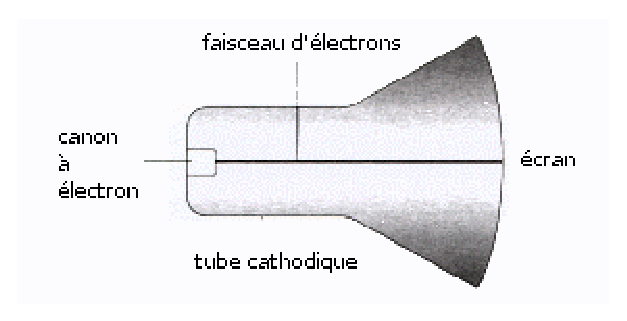
\includegraphics{electromag/tp_force_lorentz/oscilloscope_principe.xcf.eps}
\caption{Principe d'un oscilloscope}
\end{figure}
\end{center}





\section{Influence d'un aimant}


Approcher le milieu d'un petit aimant droit, ou les branches d'un
aimant en U, de ce spot.





\begin{enumerate}
\item Qu'observe-t-on ? \`A partir de ces observations, repr�senter
  pour la situation de la figure suivante la force subie par les
  �lectrons du faisceau lorsqu'ils passent au point $P$ o� l'on a
  repr�sent� le vecteur champ magn�tique.

\begin{center}
\begin{figure}[H]
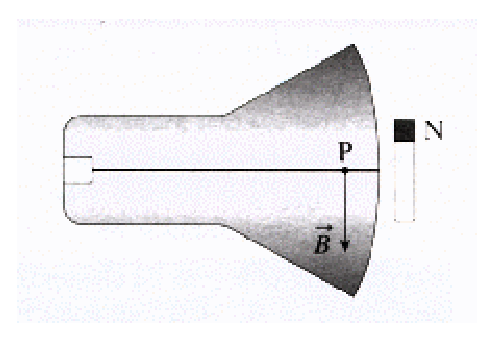
\includegraphics{electromag/tp_force_lorentz/effet_aimant_oscillo.gif.eps}
\caption{Influence d'un aimant}
\end{figure}
\end{center}

\item Quels rapprochements peut-on faire avec la force de Laplace ?

\end{enumerate}

\section{Recherche documentaire}

Rechercher des applications de la force de Lorentz.



\vressort{5}

\hrule


\section*{Annexe : spectres magn�tiques
\begin{itemize}
\item d'un aimant droit
\item et d'un aimant en U
\end{itemize}
}


\begin{center}
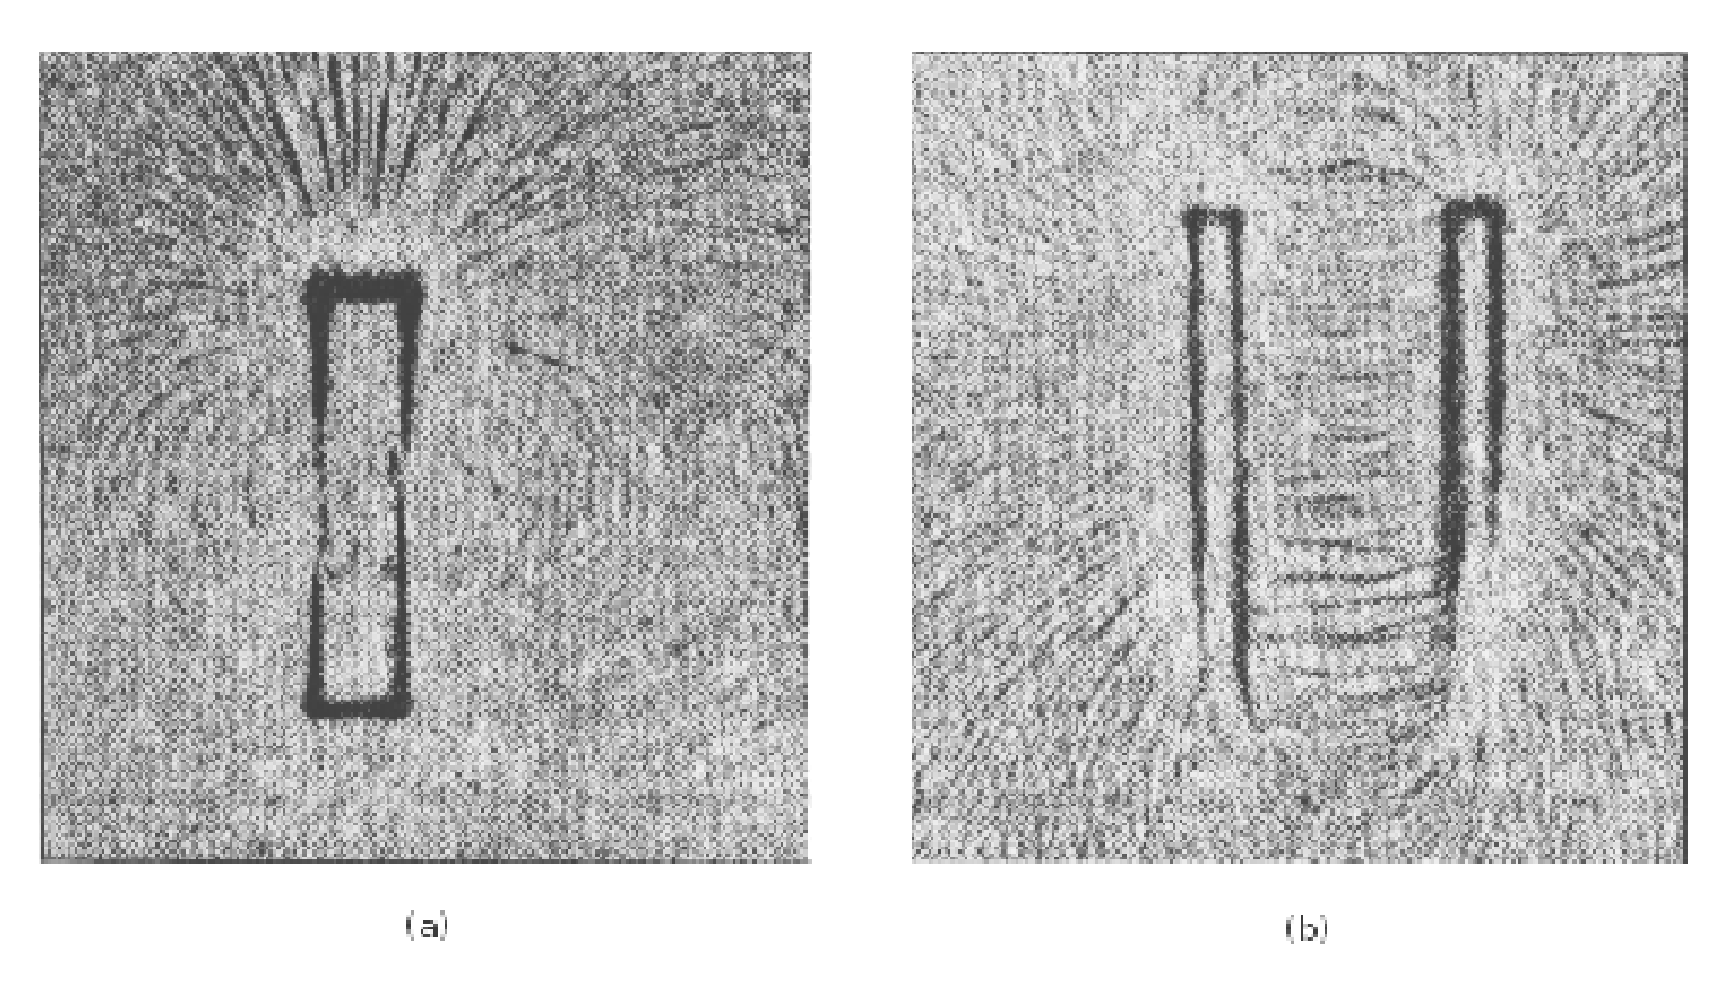
\includegraphics[width=15cm]{electromag/tp_force_lorentz/spectres.pnm.eps}
\end{center}

%\vspace{10cm}